%!Tex Root = ../main.tex
% ./Packete.tex
% ./Design.tex
% ./Vorbereitung.tex
% ./Aufgabe1.tex
% ./Aufgabe2.tex
% ./Aufgabe3.tex
% ./Aufgabe4.tex
% ./Appendix.tex

\begin{mindmap}
  \begin{mindmapcontent}
    \node (sa) at (current page.center) {Search Algorithms
      \resizebox{\textwidth}{!}{
        \begin{minipage}[t]{10cm}
          \tiny
          \begin{itemize}
            % SEARCHOVERVIEWSTART
            \item \alert{Notations:}
              \begin{itemize}
                \item \alert{Node expansion:} Look up successor nodes that are added to the frontier % considering the available incident edges
                  % generating all successor nodes considering the available edges
                \item \alert{Frontier:} Set of all nodes available for expansion (e.g. datastructures like (priority) queue or stack)
                \item \alert{Search strategy:} Defines which node is expanded next
                \item \alert{Explored set:} Set of already visited nodes %(e.g. also markings on nodes)
              \end{itemize}
            \item \alert{Criteria for search strategies:}
              \begin{itemize}
                \item \alert{Optimality:} If the strategy finds the best path (with the lowest path cost)
                \item \alert{Completeness:} If the strategy is guaranteed to find a path to a target node when there is one
                \item \alert{Time complexity} and \alert{Space complexity}
              \end{itemize}
            \item \alert{States of nodes:}
            \begin{itemize}
              \item \alert{not marked}, nodes not seen by the algorithm
              \item \alert{marked}, nodes get marked as soon as they get added to the frontier
              \item \alert{visited}, nodes are visited as soon as they get taken out of the frontier
            \end{itemize}
            % SEARCHOVERVIEWEND
          \end{itemize}
        \end{minipage}
      }
    }
    % SEARCHSTART1
    child {
      node (generalsearch) {General Search
        \resizebox{\textwidth}{!}{
          \begin{minipage}[t]{8cm}
            \begin{itemize}
              \item distinction between tree search and graph search is not rooted in the fact whether the problem graph is a tree or a general graph. It is \alert{always assumed} you're dealing with a \alert{general graph}
              \item The \alert{distinction} lies in the \alert{traversal pattern} that is used to search through the graph, which can be graph-shaped or tree-shaped
              \begin{itemize}
                \item If one is dealing with a \alert{tree-shaped problem}, both algorithm variants lead to equivalent results. So one would pick the simpler tree search variant.
              \end{itemize}
            \end{itemize}
          \end{minipage}
        }
      }
      child {
        node (ts) {Tree-based search
          \resizebox{\textwidth}{!}{
            \begin{minipage}[t]{8cm}
              \begin{itemize}
                \item nodes are possibly \alert{visited multiple times} (if there are multiple directed paths to a node rooting in the start node), possible leading even to \alert{infinite loops}
                % \item It will visit a state of the underlying problem graph multiple times, if there are multiple directed paths to it rooting in the start state
                % \item It is even possible to visit a state an infinite number of times if it lies on a directed loop
                \begin{itemize}
                  \item but each of this multiple visits would correspond to a different node if one would generate a tree by the nodes visited by the algorithm
                \end{itemize}
              \end{itemize}
            \end{minipage}
          }
          % \resizebox{\textwidth}{!}{
          %   \begin{minipage}[t]{11cm}
          %     \begin{algorithm}[H]
          %       \caption{\pr{Tree-Search}(problem)}
          %       % \begin{pseudo}[kw]
          %       % \fn{initialize} \tn{the} \tt{frontier} \tn{using the initial state of problem}\\
          %       % As long as \tt{frontier} \tn{is not} \cn{empty} do\\+
          %       % \fn{choose} \tn{a} \tt{leaf node} $v$ \tn{and remove it from the} \tt{frontier}\\
          %       %   if \tt{v} \tn{contains a} \cn{goal state} then\\+
          %       %     return \cn{True}\\-
          %       %     \fn{expand} \tn{the} \tt{node}\tn{, adding the resulting nodes to the} \tt{frontier}\\--
          %       % return \cn{False}
          %       % \end{pseudo}
          %       \begin{pseudo}[kw]
          %       \fn{initialize} \tn{the} \tt{frontier} \tn{using the initial state of problem}\\
          %       As long as \tt{frontier} \tn{is not} \cn{empty} do\\+
          %       \fn{choose} \tn{a} \tt{leaf node} \tn{and remove it from the} \tt{frontier}\\
          %         if \tt{node} \tn{contains a} \cn{goal state} then\\+
          %           return \cn{Solution}\\-
          %           \fn{expand} \tn{the} \tt{node}\tn{, adding the resulting nodes to the} \tt{frontier}\\--
          %       return \cn{Failure}
          %       \end{pseudo}
          %     \end{algorithm}
          %     \sourcesone
          %   \end{minipage}
          % }
        }
      }
      child {
        node (gs) {Graph-based search
          \resizebox{\textwidth}{!}{
            \begin{minipage}[t]{8cm}
              \begin{itemize}
                \item Keeps a \alert{explored set} and avoids the problem of tree-based search
                \item \alert{exponential memory requirements} in the worst case
              \end{itemize}
            \end{minipage}
          }
          % \resizebox{\textwidth}{!}{
          %   \begin{minipage}[t]{12cm}
          %     \begin{algorithm}[H]
          %       \caption{\pr{Graph-Search}(problem)}
          %       \begin{pseudo}[kw]
          %       \fn{initialize} \tn{the} \tt{frontier} \tn{using the initial state of problem}\\
          %       \fn{initialize} \tn{the} \tt{explored set} \tn{to be empty}\\
          %       As long as \tt{frontier} \tn{is not} \cn{empty} do\\+
          %       \fn{choose} \tn{a} \tt{leaf node} \tn{and remove it from the} \tt{frontier}\\
          %         if \tt{node} \tn{contains a} \cn{goal state} then\\+
          %           return \cn{True}\\-
          %           \fn{add} \tn{the node to the} \tt{explored set}\\
          %           if \tt{node} \tn{not in the} \tt{frontier} \tn{or} \tt{explored set} then \\+
          %             \fn{expand} \tn{the} \tt{node}\tn{, adding the resulting nodes to the} \tt{frontier}\\---
          %       return \cn{False}
          %       \end{pseudo}
          %     \end{algorithm}
          %   \end{minipage}
          % }
        }
      }
    }
    % SEARCHEND1
    % SEARCHSTART2
    child {
      node {Uninformed Search Algorithms
        \resizebox{\textwidth}{!}{
          \begin{minipage}[t]{8cm}
            \begin{itemize}
              \item  Rigid procedure with no knowledge of the cost of a given node to the goal (e.g. \alert{no heuristic function} $h(v)$), only uses other currently available knowledge (e.g. \alert{path-cost function} $g(v)$ or e.g. \alert{depth function} $d(v)$)
            \end{itemize}
          \end{minipage}
        }
      }
      child {
        node (ucs) {Uniform-Cost Search
          \resizebox{\textwidth}{!}{
            \begin{minipage}[t]{10cm}
              \begin{itemize}
                \item FIFO datastructure (FIFO-queue) gets replaced by \alert{priority queue} 
                \item expands node $v$ from the frontier with \alert{lowest path costs} $g(v)$
                \item generalization of \alert{Breadth-First Search}, where edge weights can have \alert{different values}
                \item special case of \alert{Best-First Search}, where $f(v) = g(v)$
                \item special case of \alert{A$^*$ Search}, where $h(v) = 0$ and thus $f(v) = g(v) + h(v) = g(v)$
                \begin{itemize}
                  \item if all edge weights would be $1$, then a node would have depth $k$ exactly when it's path costs would be $k$. 
                  \item then the expansion criteria would therefore be the same as for BFS, beacuse a node would have minimal depth exactly when it would have minimum path costs
                \end{itemize}
                \item is a modification of \alert{Dijkstra's Algorithm} which is focused on searching a \alert{single shortest path} in terms of \alert{cost} from the \alert{root node} to a \alert{target node} rather than finding the shortest path to every node
                \begin{itemize}
                  \item it does this by stopping as soon as the target node is found
                  \item it is applicable for both \alert{explicit graphs} and \alert{implicit graphs}, it doesn't need the entire graph as input
                \end{itemize}
                \item is \alert{complete}, provided that the branching factor is finite and \alert{optimal}
                \item \alert{Time complexity:} $O(b^{1+\left\lfloor \frac{C}{\epsilon}\right\rfloor})$
                \item \alert{Space complexity:} $O(b^{1+\left\lfloor\frac{C}{\epsilon}\right\rfloor})$, priority queue is filled gradually
              \end{itemize}
            \end{minipage}
          }
        }
        child {
          node (dijkstra) {Dijkstra's Algorithm
            \resizebox{\textwidth}{!}{
              \begin{minipage}[t]{8cm}
                \begin{itemize}
                  \item determines the \alert{shortest path} in terms of \alert{cost} from the \alert{root node} to \alert{every other node}
                  \item there is \alert{no target node}, processing continues until all nodes have been removed from the priority queue, i.e. until shortest paths to all nodes (not just a target node) have been determined
                  \item is only applicable in \alert{explicit graphs} where the entire graph is given as input
                  \item \alert{Time complexity:} always more time consuming than UCS
                  \item \alert{Space complexity:} adds all nodes to the priority queue at the beginnging with infinite cost
                \end{itemize}
              \end{minipage}
            }
          }
        }
        child {
          node (rbfs) {Breadth-First Search
            \resizebox{\textwidth}{!}{
              \begin{minipage}[t]{10cm}
                \begin{itemize}
                  \item \alert{FIFO} datastructure (FIFO-\alert{queue})
                  \item expands node $v$ from the frontier with \alert{lowest depth} $d(v)$
                  \item special case of \alert{Uniform-Cost Search} where all edge weights have \alert{no value}
                  \item special case of \alert{Best-First Search}, where $f(v) = d(v)$
                  \item \alert{complete}, provided that the branching factor is finite and \alert{optimal}, provided every edge has identical, non-negative weights
                  \item \alert{Time complexity:} $O({\mid} V{\mid}+{\mid} E{\mid})$, $b + b^2 + \ldots + b^d\in O(b^d)$ is the maximal number of nodes expanded
                  \begin{itemize}
                    \item If the algorithm were to apply the goal test to nodes when selected for expansion rather than when generated, the whole layer of nodes at depth $d$ would be expanded before the goal was detected and the time complexity would be $O(b^{d+1})$
                  \end{itemize}
                  \item \alert{Space complexity:}
                  \begin{itemize}
                    \item \alert{tree based:} $O({\mid} V{\mid}) = O(b^d)$ for the frontier%, every explored node is kept in memory
                    \item \alert{graph based:} $O(b^d)$ for the frontier and $O(b^{d-1})$ for the explored set
                  \end{itemize}
                  % \item \alert{Time complexity:} the maximal number of nodes expanded is $b+b^{2}+b^{3}+\ldots +b^{d}\in O(b^{d})$
                  % \item \alert{Space complexity:} Every node generated is \alert{kept in memory}. Therefore space needed for the \alert{frontier} is $O(b^d)$ and for the \alert{explored set} $O(b^{d-1})$
                  \item \href[page=98]{\lpathgraph{Graphentheorie_all_in_one_with_go_back.pdf}}{example}
                \end{itemize}
              \end{minipage}
            }
            \resizebox{\textwidth}{!}{
              \begin{minipage}[t]{10.5cm}
                \bfs
              \end{minipage}
            }
          }
          child {
            node (bidirectional) {Bidirectional Search}
          }
        }
      }
      child {
        node (dfs) {Depth-First Search
          \resizebox{\textwidth}{!}{
            \begin{minipage}[t]{18cm}
              \begin{itemize}
                \item \alert{LIFO} datastracture (\alert{stack})
                \item expands node $v$ from the frontier with \alert{greatest depth} $d(v)$
                \item special case of \alert{Best-First Search}, where $f(v) = -d(v)$
                \item in general, the path found is \alert{not optimal} and \alert{completeness} can be guaranteed \alert{only for graph-based search} and \alert{finite graphs}
                \item \alert{Time complexity:}
                  \begin{itemize}
                    \item \alert{graph-based:} $O({\mid} V{\mid}+{\mid} E{\mid})$, search bounded by the number of nodes (might be infinite)
                    \item \alert{tree-based:} algorithm might generate $O(b^m)$ nodes in the search tree which might be much larger than the number of nodes
                      %   \begin{itemize}
                      %     \item $m$ is the maximum length of a path in the state space
                      %   \end{itemize}
                  \end{itemize}
                  \item \alert{Space complexity:} 
                    \begin{itemize}
                      \item \alert{graph-based:} $O({\mid} V{\mid})$, in worst case, all nodes need to be stored in the explored set (no advantage over breadth-first)
                      \item \alert{tree-based:} $O(b\cdot m)$, needs to store only the nodes along the path from the root to the leaf node. Once a node has been expanded, it can be removed from memory as soon as all its descendants have been fully explored
                    \end{itemize}
                  \item \href[page=102]{\lpathgraph{Graphentheorie_all_in_one_with_go_back.pdf}}{example}
                  \item \underline{For every node $v$ two points in time are defined:}
                    \begin{itemize}
                      \item \alert{$t_{v,1}$:} Point in time, when $v$ gets in the marked state
                      \item \alert{$t_{v,2}$:} Point in time, when $v$ gets in the visited state
                    \end{itemize}
                  \item in the DFS-Search-Tree a node $v$ is in the subtree of a node $u$ \alert{iff} the intervall $[t_{v,1}$, $t_{v,2}]$ is fully contained in the intervall $[t_{u,1}, t_{u,2}]$
                  \item \alert{Classification of edges:} $uv$ is 
                    \begin{itemize}
                      \item a \alert{tree edge}, if $v$ was discovered from $u$
                        \begin{itemize}
                          \item $u$ is in marked state, $v$ is in not marked state when looking at $uv$
                        \end{itemize}
                      \item a \alert{backward edge}, if $v$ is a predecessor node of $u$
                        \begin{itemize}
                          \item $u$ is in marked state, $v$ is in marked state when looking at $uv$
                          \item $t_{v,1}<t_{u,1}<t_{u,2}<t_{v,2}$
                        \end{itemize}
                      \item a \alert{forward edge}, if $v$ is a successor node of $u$ 
                        \begin{itemize}
                          \item $u$ is in marked state, $v$ is in visited state when looking at $uv$
                          \item $t_{u,1}<t_{v,1}<t_{v,2}<t_{u,2}$, $\boxed{t_{u,1}<t_{v,1}}$
                        \end{itemize}
                      \item a \alert{cross edge}, if it is neither of all above
                        \begin{itemize}
                          \item $u$ is in marked state, $v$ is in visited state when looking at $uv$
                          \item $t_{v,1}<t_{v,2}<t_{u,1}<t_{u,2}$, $\boxed{t_{v,1}<t_{u,1}}$
                        \end{itemize}
                      \item \href[page=34]{\lpathdfssearch}{example}
                    \end{itemize}
                    \item more about DFS-Search-Trees \href[page=35]{\lpathdfssearch}{here}
                \end{itemize}
                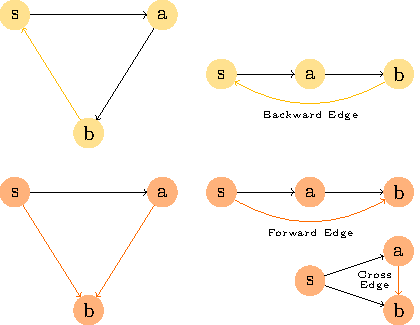
\includegraphics[width=0.5\textwidth, center]{./figures/dfs.pdf}
            \end{minipage}
          }
          \resizebox{\textwidth}{!}{
            \begin{minipage}[t]{11cm}
              \dfs
            \end{minipage}
          }
        }
        child {
          node {Recursive Depth-First Search
            \resizebox{\textwidth}{!}{
              \begin{minipage}[t]{11cm}
                \dfsrec
              \end{minipage}
            }
          }
        }
        child {
          node {Depth-Limited Search}
          child {
            node {Iterative-Deepening Search}
          }
        }
      }
    }
    % SEARCHEND2
    % SEARCHSTART3
    child {
      node {Informed Search Algorithms
        \resizebox{\textwidth}{!}{
          \begin{minipage}[t]{8cm}
            \begin{itemize}
              \item Knowledge of the worth of expanding a node $v$ is given in the form of an \alert{evaluation function} $f(v)$, which assigns a real number to each node
              \item Often $f(v)$ includes a \alert{heuristic function} $h(v)$ as a component, which estimates the costs of the cheapest path from $v$ to the goal
            \end{itemize}
          \end{minipage}
        }
      }
      child {
      node {Local Search Algorithms
        \resizebox{\textwidth}{!}{
          \begin{minipage}[t]{8cm}
            \begin{itemize}
              \item if it is unimportant how the goal is reached, \alert{only the goal itself matters} and if in addition a \alert{quality} measure for nodes is given
              \item it operates using a \alert{single current node} (rather than multiple paths)
              \item requires little memory
            \end{itemize}
          \end{minipage}
        }
      }
      child {
        node {Hill Climbing
          \resizebox{\textwidth}{!}{
            \begin{minipage}[t]{8cm}
              \begin{itemize}
                \item Begin with a randomly-chosen configuration and \alert{improve} on it \alert{step by step}
              \end{itemize}
            \end{minipage}
          }
        }
        child {
          node {Simulated Annealing
            \resizebox{\textwidth}{!}{
              \begin{minipage}[t]{8cm}
                \begin{itemize}
                  \item \enquote{noise} is injected systematically, first a lot, then gradually less
                \end{itemize}
              \end{minipage}
            }
          }
        }
        child {
          node {Gradient Descent}
        }
      }
    }
    child {
      node {Genetic Algorithms
        \resizebox{\textwidth}{!}{
          \begin{minipage}[t]{8cm}
            \begin{itemize}
              \item Similar to \alert{evolution}, we search for solutions by three operators: \alert{mutation}, \alert{crossover}, and \alert{selection}
            \end{itemize}
          \end{minipage}
        }
      }
    }
      child {
        node (bfs) {Best-First Search 
          \resizebox{\textwidth}{!}{
            \begin{minipage}[t]{8cm}
              \begin{itemize}
                \item informed search procedure that expands the node with the \enquote{\alert{best}} $f$-value first
                \item is an instance of the general \alert{Tree-Search} algorithm in which frontier is a \alert{priority queue} ordered by an \alert{evaluation function} $f$
                \begin{itemize}
                  \item when $f$ is always correct, ones does not need to search
                \end{itemize}
              \end{itemize}
            \end{minipage}
          }
        }
        child {
          node {Greedy Search
            \resizebox{\textwidth}{!}{
              \begin{minipage}[t]{8cm}
                \begin{itemize}
                  \item A \alert{best-first} search using the \alert{heuristic function} $h(v)$ as the \alert{evaluation function}, i.e. $f(v) = h(v)$ is called a \alert{greedy search}
                  \begin{itemize}
                    % \item judge the \enquote{worth} of a node by estimating its path costs to the target node
                    \item $h(v) =$ estimated path-costs from $v$ to the target node
                    \item the only real restriction is that $h(v) = 0$ if $v$ is the target node
                  \end{itemize}
                  \item is generally \alert{incomplete} and \alert{not optimal}
                  \begin{itemize}
                    \item \alert{graph-search} version is complete only in finite graphs
                  \end{itemize}
                \end{itemize}
              \end{minipage}
            }
          }
          child {
            node (hf) {Heuristic function
              \resizebox{\textwidth}{!}{
                \begin{minipage}[t]{8cm}
                  \begin{itemize}
                    \item or simply a \alert{heuristic}
                    \item the evaluation function $f$ in \alert{greedy searches} is a heuristic function $h$ 
                    \item the heuristic is \alert{problem-specific} and \alert{focuses} the search
                    \item \alert{In AI it has two meanings:}
                    \begin{itemize}
                      \item Heuristics are \alert{fast} but in certain situations \alert{incomplete} methods for problem-solving
                      \item Heuristics are methods that \alert{improve the search} in the \alert{average-case}
                    \end{itemize}
                    \item The word heuristic is derived from the Greek word {\gyre ευρισκειν} (note also: {\gyre ευρηκα!})
                  \end{itemize}
                \end{minipage}
              }
            }
          }
        }
        child {
          node (astar) {A$^*$
            \resizebox{\textwidth}{!}{
              \begin{minipage}[t]{8cm}
                \begin{itemize}
                  \item A$^*$ combines \alert{greedy search} with the \alert{uniform-cost search}
                  \item Always expands node with lowest \alert{evaluation function} $f(v)$ first, where:
                  \begin{itemize}
                    \item $g(v) =$ actual cost from the start node to $v$
                    \item $h(v) =$ estimated cost from $v$ to the nearest target node
                    \item $f(v) = g(v) + h(v) =$ the estimated cost of the cheapest path through $v$
                  \end{itemize}
                  \item We require that for A$^*$, that $h$ is admissible (e.g. straight-line distance is admissible)
                  \begin{itemize}
                    \item $h$ is an \alert{optimistic estimate} of the costs that actually occur
                  \end{itemize}
                  \item \alert{complete}, provided that every node has a finite number of successor nodes and there exists a positive constant $\delta > 0$ such that every edge has at least weight $\delta$ and \alert{optimal}, provided that one uses the \alert{tree-based} variant
                  \begin{itemize}
                    \item for the \alert{graph-based} variant, one:
                    \begin{itemize}
                      \item either needs to consider re-opening nodes from the explored set, when a better estimate becomes known, or
                      \item one needs needs to require stronger restrictions on the heuristic estimate: it needs to be \alert{consistent}
                      \item $A^*$ can still be applied if heuristic is not consistent, but \alert{optimality is lost} in this case
                    \end{itemize}
                  \end{itemize}
                  \item \alert{Time complexity:} $O(b^d)$, exponential in the path length of the solution. More refined complexity results depend on the assumptions made, e.g. on the quality of the heuristic function
                  \item \alert{Space complexity:} $O(b^d)$, exponential in the path length of the solution. Roughly the same as that of all other graph search algorithms, as it keeps all generated nodes in memory
                \end{itemize}
              \end{minipage}
            }
          }
          child {
            node {Iterative-Deepening A$^*$ (IDA$^*$)
          %     \resizebox{\textwidth}{!}{
          %       \begin{minipage}[t]{8cm}
          %         \begin{itemize}
          %           \item the $f$-costs are used to define the cutoff (rather than the depth of the search tree)
          %         \end{itemize}
          %       \end{minipage}
          %     }
            }
          }
          child {
            node {Recursive Best First Search (RBFS)}
          }
          child {
            node {Memory-bounded A$^*$ (MA$^*$) and Simplified MA$^*$ (SMA$^*$)}
          }
          child {
            node {Admissible
              \resizebox{\textwidth}{!}{
                \begin{minipage}[t]{8cm}
                  \begin{itemize}
                    \item $h$ is admissible if the following holds for all $v$: $h(v) \le h^*(v)$
                    \begin{itemize}
                      \item $h^*(v)$ are the actual cost of the optimal path from $v$ to the target node
                    \end{itemize}
                  \end{itemize}
                \end{minipage}
              }
            }
          }
          child {
            node {Consistent
              \resizebox{\textwidth}{!}{
                \begin{minipage}[t]{8cm}
                  \begin{itemize}
                    \item A heuristic $h$ is called consistent \alert{iff} for all edges $v$ leading from $s$ to $s'\colon h(s) - h(s') \le c(v)$, where $c(v)$ denotes the weight of edge $v$
                    \item Consistent heuristics prevent the need to re-open nodes from the explored set
                    \item Consistency implies \alert{admissibility}
                  \end{itemize}
                \end{minipage}
              }
            }
          }
        }
      }
    } 
    % SEARCHEND3
    ;
  \end{mindmapcontent}
  \begin{edges}
    % SEARCHCONNECTIONSSTART
    \edge{dfs}{bidirectional}
    \edge{ts}{bfs}
    % \edge{ts}{rbfs}
    % \edge{gs}{dfs}
    \edge{astar}{ucs}
    \edge{bfs}{ucs}
    % \edge{bfs}{rbfs}
    \edge{bfs}{dfs}
    \edge{hf}{astar}
    % SEARCHCONNECTIONSEND
  \end{edges}
  % SEARCHANNOTATIONSSTART
  \annotation{dfs}{\bd}
  \annotation{rbfs}{\bd}
  \annotation{generalsearch}{\sourcesone}
  \annotation{dijkstra}{
    \resizebox{\textwidth}{!}{
      \begin{minipage}[t]{4cm}
        \cite{vineetnayak28AnswerWhatDifference2016}
      \end{minipage}
    }
  }
  % SEARCHANNOTATIONSEND
  \annotation{sa.south}{This mindmap is provided without guarantee of correctness and completeness!}
  \annotation{sa.north}{\href{/tmp/current.pdf}{go back}}
\end{mindmap}
